\subsection{Movimiento horizontal}

\subsubsection{Parámetros del sistema}

El sistema de movimiento horizontal utiliza una transmisión por correa dentada GT2 con las siguientes especificaciones:

\begin{itemize}
    \item Carga total: $m = 1.5$ kg
    \item Longitud de la correa: $L = 2.84$ m (ec. \ref{eq:longitud_correa})
    \item Diámetro de poleas: $D_p = 12$ mm y 20 dientes
    \item Radio de poleas: $r = 6$ mm = $0.006$ m
    \item Ancho de la correa: $b = 10$ mm
    \item Paso de la correa GT2: $p = 2$ mm
    \item desplazamiento lineal por revolución: $d_{rev} = 40 \frac{mm}{rev}$
\end{itemize}

\subsubsection{Cálculo de fuerzas actuantes}

\paragraph{Fuerza de aceleración}

Considerando una aceleración deseada de $a = 0.188$ m/s$^2$:

\begin{equation}
    F_a = m \cdot a = 0.32 \text{ N}
\end{equation}

\paragraph{Fuerza de fricción}

Se toma un coeficiente de fricción de 0.15 debido a que el sistema no es tan preciso y puede tener fricción de desplazamiento.

\begin{equation}
    F_f = \mu \cdot m \cdot g = 0.39 \text{ N}
\end{equation}

\paragraph{Resistencia interna de correa}
Para esto, se toma un valor empírico, considerando el largo.
\[F_{intcorrea} \approx 0.25N\]
\paragraph{Otras pérdidas}

\begin{equation}
    F_{otras}= 0.1*(F_a+F_f)=0.07N
\end{equation}

\paragraph{Fuerza total requerida}

La fuerza total que debe ejercer el motor es la suma de la fuerza de aceleración y la fuerza de fricción:

\begin{equation}
    F_{total} = F_a + F_f + F_{intcorrea} + F_{otras} = 1.05 \text{ N}
\end{equation}

\subsubsection{Torque Requerido en el Motor}

El torque necesario en el eje del motor se calcula multiplicando la fuerza total por el radio de la polea:

\begin{equation}
    T_{req} = F_{total} \cdot r = 0.013\text{ N·m}
\end{equation}

Para garantizar un funcionamiento confiable del sistema, se aplica un factor de seguridad de 2.5:

\begin{equation}
    T_{motor} = T_{req} \cdot FS = 0.013 \cdot 2.5
\end{equation}

\subsubsection{Selección del motor}

Considerando el torque calculado con factor de seguridad, se selecciona el motor paso a paso  \textbf{Nema 17 medium} que posee  0.35Nm a 24V y 1.8A. 

\subsubsection{Resolución de posicionamiento}

Con microstepping de 8 pasos (configuración típica con driver TB6600):

\begin{equation}
    \text{Pasos totales/rev} = 200 \cdot 8 = 1600 \text{ pasos/rev}
\end{equation}

\begin{equation}
    \text{Resolución} = \frac{d_{rev}}{\text{Pasos totales/rev}} = \frac{40}{1600} = 0.025 \text{ mm/paso}
\end{equation}

\subsubsection{Velocidad máxima del sistema}

Considerando una velocidad máxima de 0.25 \(\frac{m}{s}\) se tiene que la velocidad angular máxima del motor es:

\begin{equation}
    n_{max} = \frac{250 \frac{mm}{s} \cdot 60 \text {s}}{40 \frac{mm}{rev}} = 375 \text{ rpm}
\end{equation}
Como se puede observar en la figura \ref{fig:Curva_din_nema17medium} para la velocidad máxima se cumple con el torque necesario.
\begin{figure}[H]
    \centering
    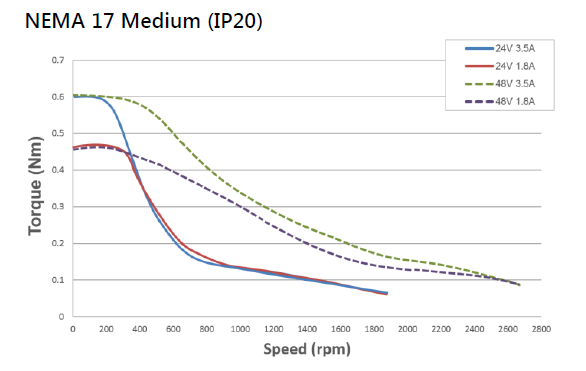
\includegraphics[width=0.65\textwidth]{img/nema17_medium.png}
    \caption{\textit{Curva dinámica torque-velocidad del motor paso a paso NEMA 17 para el prototipo.}}
    \label{fig:Curva_din_nema17medium}
\end{figure}
Como se cuentan con motores paso a paso que poseen 0.22Nm de torque se opta utilizar una configuración de dos motores, por lo que cada polea está acoplada a un motor. De esta manera se obtiene el torque final necesario a aplicar como la suma de los torques de ambos motores.